\section{Ponteiros}
%==================================================================================
\begin{frame}
\frametitle{Ponteiros e vetores}

\begin{block}{Vetores}
\justifying
Vetores são sequências de elementos de um tipo de dado, armazenados em posições contíguas de memória, distribuídas em um número predeterminado de dimensões.
\end{block}

	\begin{figure}[h]
		\centering
		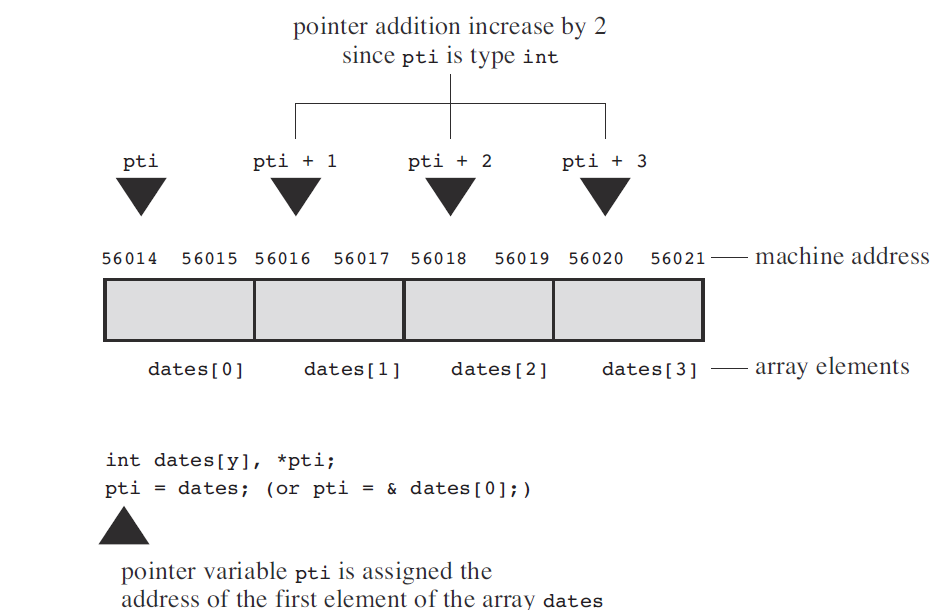
\includegraphics[width=0.75\textwidth]{Imagens/Imag02.png}
		%\caption*{Linguagem Python.}
	\end{figure}


\end{frame}

%==================================================================================


\begin{frame}[fragile]
  \frametitle{Referenciando os elementos dos vetores}
  
\begin{block}{Vetores}
\justifying
As referências aos elementos dos vetores são implementadas através da aritmética de ponteiros.
\end{block}

  \begin{block}{Exemplo: vetor 1-d}
  \begin{lstlisting}
#include <stdio.h>
#include <stdlib.h>

int main()
{
    int vet[5]={10,2,3,5,14};
    int *ptr_vet;

    ptr_vet=&vet;

    printf("%d\n",vet[1]);
    printf("%d\n",*(ptr_vet+1));

    return 0;
}
  \end{lstlisting}
  \end{block}
\end{frame}
%==================================================================================

\begin{frame}[fragile]
  \frametitle{Referenciando os elementos dos vetores}

  \begin{block}{Exemplo: vetor 2-d}
  \begin{lstlisting}
#include <stdio.h>
#include <stdlib.h>

int main()
{
    int vet[3][3]={{10,2,3},{5,14,-3},{9,6,4}};
    int *ptr_vet;

    int row=3,col=3,i,j;

    ptr_vet=&vet;
    i=1;
    j=2;

    printf("%d\n",vet[i][j]);

    printf("%d\n",*(ptr_vet + row*i + j));

    return 0;
}

  \end{lstlisting}
  \end{block}
\end{frame}